\documentclass[12pt,a4paper]{article}

\usepackage{t1enc}
\usepackage[utf8]{inputenc}
\usepackage[magyar]{babel}
\usepackage{makeidx}
\usepackage{natbib}
\usepackage{enumitem}
\usepackage[version=4]{mhchem}
\usepackage{graphicx}
\usepackage{tabu}
\usepackage{makecell}

\usepackage{tikz}
\usetikzlibrary{positioning}

\author{Gáspár Tamás}
\title{A PageRank algoritmus}
\date{}

% számláló és formázás definícióknak: \begin{definicio}
\newcounter{definicioszam}
\newenvironment{definicio}[1]
{{\medskip}\noindent \stepcounter{definicioszam}
{\bfseries{\thedefinicioszam. Definíció: #1\\[1ex]}}}{\bigskip }

%számláló és formázás tételeknek: \begin{tetel}
\newcounter{tetelszam}
\newenvironment{tetel}[1]
{{\medskip}\noindent \stepcounter{tszam}
{\bfseries{\thetetelszam. Tétel: #1\\[1ex]}}}{\bigskip }

\begin{document}

%FŐOLDAL ------------------------------------------------------------------

%intézet
\thispagestyle{empty}
\centerline{\textsc{\Large{Szegedi Tudományegyetem}}}
\vspace{0.3 cm}
\centerline{\textsc{\Large{Természettudományi és Informatikai Kar}}}

\vspace*{2 cm}

\centerline{\textsc{\Large{Bólyai Intézet}}}
\vspace{0.3 cm}
\centerline{\textsc{\Large{Sztochasztika tanszék}}}

\vspace{3 cm}

%cím
\centerline{\LARGE{A PageRank algoritmus}}
\vspace{0.5 cm}
\centerline{\Large{\textsc{Szakdolgozat}}}

\vspace{3 cm}

%készítő és témavezető táblázat
\begin{center}
	\begin{tabu} to \textwidth { X[l]  X[r] }
		\makecell[l]{Készítette: Gáspár Tamás \\ Matematika BSc hallgató} &
		 \makecell[r]{Témavezető: Dr. Kevei Péter \\ Egyetemi docens \\ Sztochasztika tanszék} \\
	\end{tabu}
\end{center}

\vspace{3 cm}

\centerline{\Large{\textsc{Szeged, 2019}}}

%tartalomjegyzék oldala -------------------------------------------------
\newpage
\thispagestyle{empty}

\tableofcontents

%tényleges kezdet --------------------------------------------------------
\newpage
\setcounter{page}{1}
\fontsize{12}{16}\selectfont

\section{Bevezető}

Dolgozatom témája a PageRank algoritmus, melynek legfőbb alkalmazási területe az internetes weboldalak bizonyos szempontok szerinti rangsorolása.

Ebben a fejezetben röviden ismertetem a PageRank algoritmus történetét és megemlítek egy PageRank számolásához használható, általam készített programot. A második fejezetben a PageRank algoritmus tárgyalásához szükséges alapvető fogalmakat és definíciókat vezetek be. 

\subsection{A PageRank algoritmus története}

A PageRank algoritmust Larry Page és Sergei Brin alkották meg 1998-ban, a Standford Egyetem hallgatóiként. Arra kerestek megoldást, hogy miként lehet az akkoriban robbanásszerű növekedésnek induló internetet weboldalait továbbra is rangsorolni, mivel látszott, hogy az akkor alkalmazott keresőmotorok erre már hamarosan nem lesznek képesek.

Úgy gondolták, hogy a rangsorolás alapja az internet hiperlink struktúrája kell hogy legyen. Feltették, hogy ha egy oldal linkel egy másikra, az kifejezi azt, hogy az oldal készítői megbíznak a linkelt oldalban, ezért az algoritmusukat úgy építették fel, hogy egy oldal fontossága (ezt szintén PageRanknak nevezik) attól függ, hogy mennyi és milyen fontos oldalak linkelnek rá.

Larry Page és Sergei Brin találmánya olyan jól alkalmazhatónak bizonyult, hogy Google néven saját vállalkozást alapítottak. A cég keresőmotorjának alapja máig a PageRank algoritmus, skálázhatóságát mutatja, hogy a Google ma már több mint 130 billió weboldalt indexel. 

\subsection{PageRank program}

Dolgozatomhoz grafikus felhasználói felülettel ellátott asztali alkalmazást is készítettem, Java nyelven. Ez a program képes előre megadott oldalszámú webet különböző paraméterek alapján véletlenszerűen generálni, majd ehhez PageRankot számolni. A 150 oldalnál kisebb méretű webekhez tartozó mátrixokat meg is tudja jeleníteni.

A program és annak forráskódja is letölthető a következő oldalról:

\vspace{0.3 cm}
\textit{https://github.com/Gtomika/PageRank/releases/tag/v4.1}
\vspace{0.3 cm}

 A futtatáshoz a számítógépen telepítve kell hogy legyen a Java.

\section{Alapfogalmak és definíciók}

\subsection{Linkek, web}

Ahhoz hogy a PageRank algoritmust definiálhassam, először a web fogalmát kell bevezetni.

\begin{definicio}{Linkhalmaz}
	Legyen V a weboldalak halmaza. Ekkor $L \subset V \times V$ \textbf{linkhalmaz}ban $(v_1,v_2)$ ($v_1, v_2 \in V$ és $v_1 \ne v_2$) pontosan akkor van benne ha $v_1$ linkel $v_2$-re. 
\end{definicio}

\begin{definicio}{Web}
	Legyen V a weboldalak halmaza, L pedig az ehhez tartozó linkhalmaz. Ekkor a \textbf{web} egy irányított gráf, melynek csúcsai V elemei, élei pedig L elemei, ahol ha $v_1, v_2 \in V$ és $(v_1,v_2) \in L$, akkor az él $v_1$-ből $v_2$-be mutat. 
\end{definicio}

\begin{figure}[h]
	\centering
	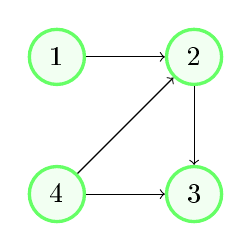
\begin{tikzpicture}[
	roundnode/.style={circle, draw=green!60, fill=green!5, very thick, minimum size=7mm},
	]
	\centering
	%Nodes
	\node[roundnode]      (c1)                     {1};
	\node[roundnode]      (c2)       [right=of c1] {2};
	\node[roundnode]      (c3)       [below=of c2] {3};
	\node[roundnode]      (c4)       [below=of c1] {4};
	
	%Lines
	\draw[->] (c1) -- (c2);
	\draw[->] (c2) -- (c3);
	\draw[->] (c4) -- (c2);
	\draw[->] (c4) -- (c3);
	\end{tikzpicture}
	\caption{Egy 4 oldalból álló web}
\end{figure}

A linkhalmaz definíciójában lévő egyszerűsítő feltétel amely nem engedi, hogy egy oldal saját magára linkel, azért tehető meg, mert bár egy valós web esetén ez lehetséges, de a PageRank algoritmusba az ilyen típusú linkek nem számítanak bele, ez ugyanis lehetővé tenné, hogy egy oldal egyszerűen növelje a saját értékelését azzal, hogy sokszor linkel önmagára. 

\subsection{A PageRank definíciója}

Egy oldal fontossága azon múlik, hogy mennyi oldal linkel rá, és hogy ezek milyen fontosak. A linkelő oldalak fontosságára azért van szükség, mert enélkül egy oldaltulajdonos tudná úgy növelni a weboldalának fontosságát, hogy rengeteg oldalt hoz létre, melyek mind linkelnek egymásra és a saját oldalára (ezt link farmnak nevezik \cite{langvillebook}).

Az egy oldal fontosságát leíró pozitív valós számot is szokás az algoritmushoz hasonlóan PageRanknak nevezni. Egy webet el lehet úgy is képzelni, mint az oldalak demokráciáját ahol minden oldalnak szavazata van és ezt a szavazatot (és még a kapott szavazatokat is) továbbosztja úgy, hogy linkel a többi oldalra.

\begin{definicio}{Weboldal PageRankja}
	Legyen adott egy web, V az oldalak, L a linkek halmaza.
	Legyen $v_i \in V$ oldal PageRankja $r(v_i)$, az oldalról kimenő linkek száma pedig $ |\ v_i |\ $. 
	
	Jelölje $B_i \subset V$ azon oldalak halmazát amelyen linkelnek $v_i$-re, azaz
	\[B_i = \{ v_j \in V: \exists l \in L, \quad l = (v_j,v_i) \} \]
	
	Ekkor bármely $v_i$ oldal PageRankját megkapjuk a következő módon:
	
	\[ r(v_i) = \sum_{v_j \in B_i} \frac{r(v_j)}{ |\ v_j|\ } \]
\end{definicio}

A definícióban megjelenik az is, hogy egy oldalnak mennyi kimenő linkje van. Minél több oldalra linkel, annál kevesebbet fog számítani az ő linkjének értéke. Ez ellensúlyozza a már említett link farmokat.

A szummában szereplő oldalak egyikénél sem lehet a kimenő linkek száma nulla, mert mindegyik oldal eleme a $B_i$ halmaznak, azaz legalább $v_i$-re linkelnek.

\bigskip

A PageRank definíciója tehát rekurzív. Egy oldal rangjának meghatározásához minden rá linkelő oldal rangját ismernünk kell. Ha a webünk $n$ db oldalt tartalmaz, akkor a definíció meghatároz $n$ db lineáris egyenletet.

A cél az, hogy olyan algoritmust adjunk meg, amely egyrészt pontosan meghatározza minden oldal PageRankját, másrészt nagyon nagy $n$-re is hatékonyan működik, mind idő-, mind tárigény szempontjából. 

\begin{definicio}{Linkmátrix}
	
\end{definicio}


\section{Hivatkozások}

%hivatkozások ---------------------------------------------------------
\begin{thebibliography}{10}
	\bibitem{langvillebook}
	Amy N. Langville, Carl D. Meyer.
	\textit{Google's PageRank and Beyond: The Science of Search Engine Rankings.}
	Princeton University Press, 2012
\end{thebibliography}

\end{document}